\documentclass[11pt]{article}
\usepackage[utf8]{inputenc}
\usepackage[spanish]{babel}
\usepackage{amsmath,amssymb,amsthm}
\usepackage{graphicx}
\usepackage[margin=2.5cm]{geometry}
\usepackage{enumitem}

\newtheorem*{definicion}{Definición}
\newtheorem*{ejemplo}{Ejemplo}
\newtheorem*{observacion}{Observación}

\title{Semana 7 -- Materia}
\author{Tutorías -- Introducción al Cálculo}
\date{21/9--25/9/2026}

\begin{document}
\maketitle

\section{Transformaciones de funciones}

Dada una función real $f$, podemos construir nuevas funciones a partir de ella
aplicando ciertas operaciones simples (sumar una constante, multiplicar por una
constante, cambiar el signo de la variable, etc.). Cada una de estas operaciones
tiene un efecto geométrico muy concreto sobre el gráfico de $f$: una traslación,
una reflexión o un escalamiento. En esta sección repasamos estas transformaciones
a través de ejemplos, tal como se presentan en el libro.

\subsection{Reflexión respecto al eje $X$: $-f$}

Si $f$ es una función real, definimos la función $-f$ por $(-f)(x) = -f(x)$.
Geométricamente, el gráfico de $-f$ se obtiene reflejando el gráfico de $f$
respecto al eje $X$: si $(x,y) \in f$ entonces $(x,-y) \in -f$.

\begin{ejemplo}
Sea $f(x) = 2x+5$. Entonces $(-f)(x) = -f(x) = -2x-5$. Los gráficos de $f$ y de
$-f$ son simétricos respecto al eje $X$.

\begin{center}
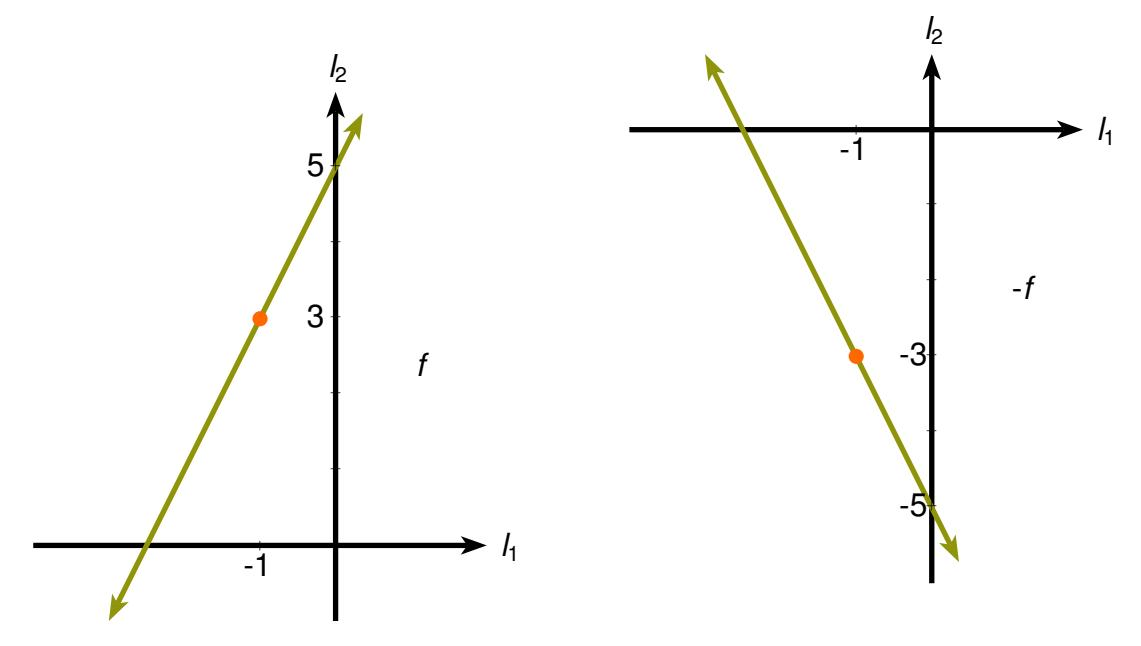
\includegraphics[width=0.55\textwidth]{img/_page_139_Figure_7.jpeg}
\end{center}
\end{ejemplo}

\subsection{Desplazamiento vertical: $f+c$}

Si $c \in \mathbb{R}$, la función $f+c$ se define por $(f+c)(x) = f(x)+c$. El
gráfico de $f+c$ es el gráfico de $f$ desplazado en $c$ unidades respecto al
eje $Y$: si $(x,y) \in f$ entonces $(x, y+c) \in f+c$.

\begin{ejemplo}
Sea $f(x) = x^2$. Entonces $(f+5)(x) = f(x) + 5 = x^2+5$: el gráfico de $f+5$
es el de $f$ desplazado 5 unidades hacia arriba.

\begin{center}
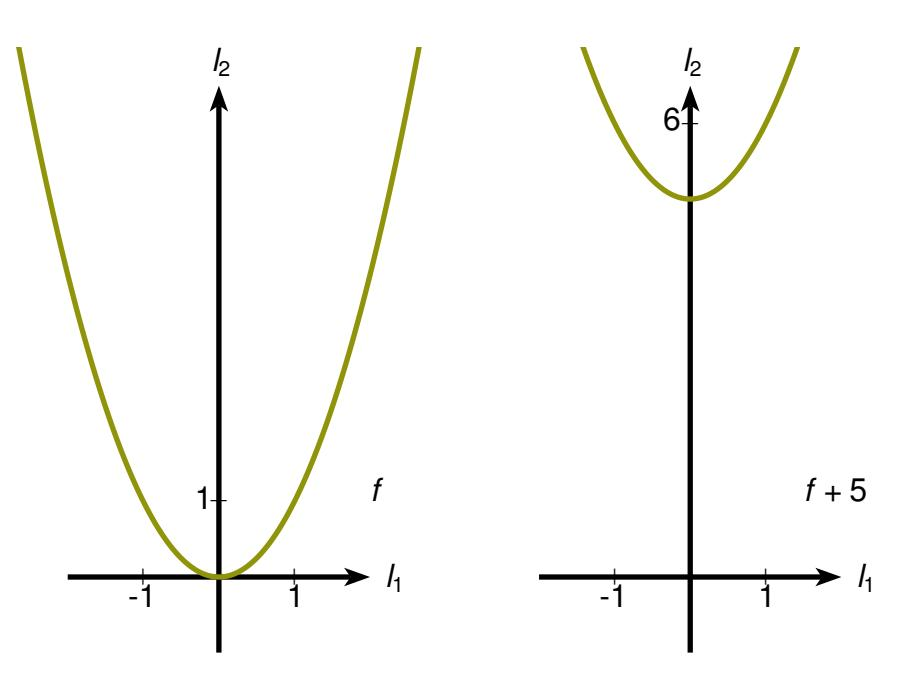
\includegraphics[width=0.55\textwidth]{img/_page_140_Figure_3.jpeg}
\end{center}
\end{ejemplo}

\subsection{Escalamiento vertical: $c\cdot f$}

Si $c \in \mathbb{R}$, la función $c\cdot f$ se define por $(cf)(x) = c\,f(x)$.
El gráfico de $cf$ se obtiene del de $f$ ampliando (si $|c|>1$) o comprimiendo
(si $|c|<1$) verticalmente en un factor $c$: si $(x,y) \in f$ entonces
$(x, cy) \in cf$.

\begin{ejemplo}
Sea $f(x) = \sqrt{1-x^2}$. Entonces $(4f)(x) = 4f(x) = 4\sqrt{1-x^2}$: el
gráfico de $4f$ es el de $f$ ampliado 4 veces respecto al eje $Y$.

\begin{center}
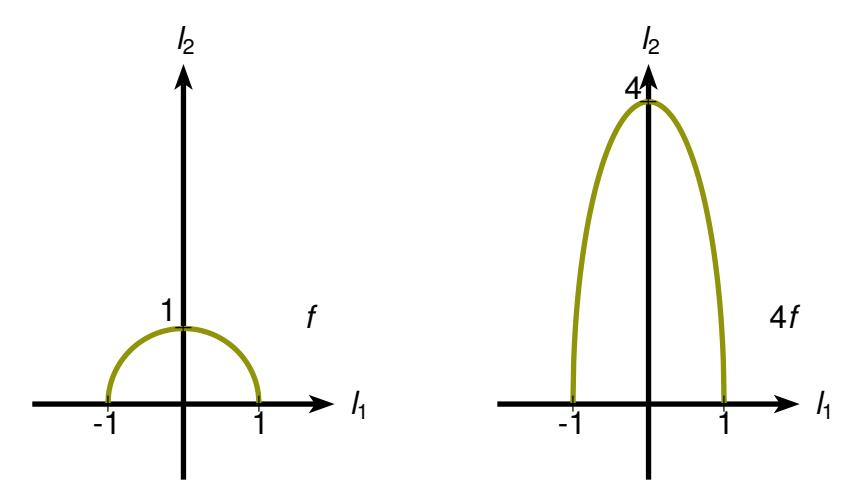
\includegraphics[width=0.55\textwidth]{img/_page_140_Figure_8.jpeg}
\end{center}
\end{ejemplo}

\subsection{Valor absoluto de una función: $|f|$}

La función $|f|$ se define por $|f|(x) = |f(x)|$. Su gráfico coincide con el
de $f$ donde $f(x) \ge 0$, y con el de $-f$ donde $f(x) < 0$: la parte negativa
de $f$ se refleja respecto al eje $X$. Es decir, si $(x,y) \in f$ entonces
$(x,|y|) \in |f|$.

\begin{ejemplo}
Sea $f(x) = 2x$. Entonces $|f|(x) = 2|x|$.

\begin{center}
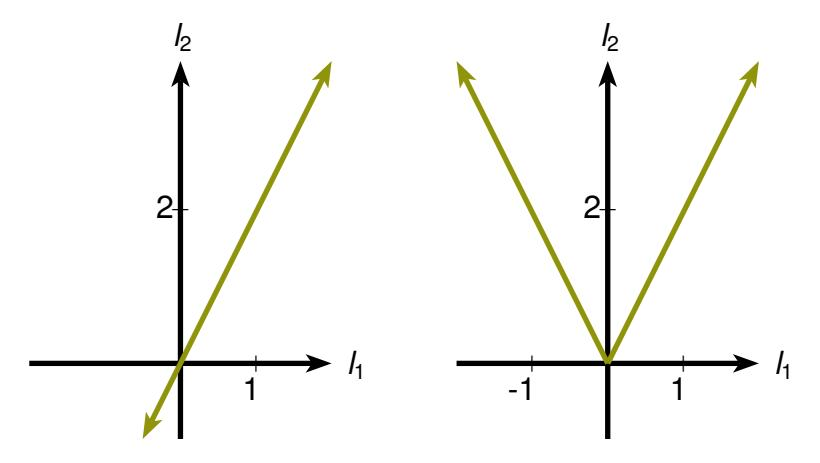
\includegraphics[width=0.55\textwidth]{img/_page_141_Figure_5.jpeg}
\end{center}
\end{ejemplo}

\subsection{Desplazamiento horizontal: $f(x-c)$}

Si $g(x) = f(x-c)$ con $c \in \mathbb{R}$, el gráfico de $g$ es el gráfico de
$f$ trasladado horizontalmente en $c$ unidades: si $(x-c,y) \in f$ entonces
$(x,y) \in g$. Si $c>0$ la traslación es hacia la derecha; si $c<0$, hacia la
izquierda.

\begin{ejemplo}
Sea $f(x) = x^2$ y $g(x) = f(x-2) = (x-2)^2$. El gráfico de $g$ es el de $f$
trasladado 2 unidades hacia la derecha.

\begin{center}
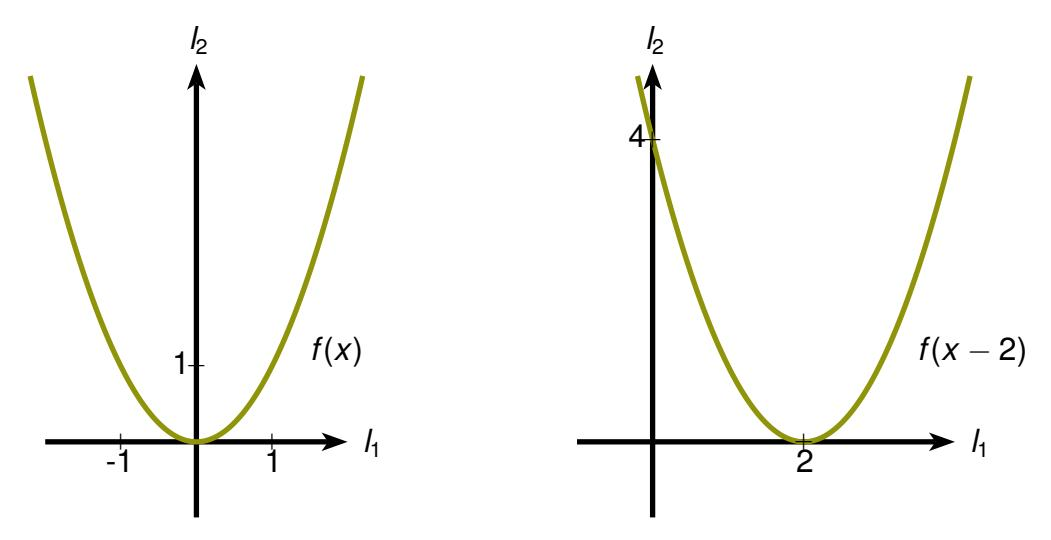
\includegraphics[width=0.55\textwidth]{img/_page_141_Figure_10.jpeg}
\end{center}
\end{ejemplo}

\subsection{Escalamiento horizontal: $f(cx)$}

Si $g(x) = f(cx)$ con $c \in \mathbb{R}$, $c \neq 0$, el gráfico de $g$ se
obtiene comprimiendo (si $|c|>1$) o expandiendo (si $|c|<1$) horizontalmente el
gráfico de $f$: si $(cx,y) \in f$ entonces $(x,y) \in g$.

\begin{ejemplo}
Sean $f(x) = \sqrt{1-x^2}$ y $g(x) = f(2x) = \sqrt{1-4x^2}$. El gráfico de $g$
es el de $f$ comprimido en un factor 2 respecto al eje $X$.

\begin{center}
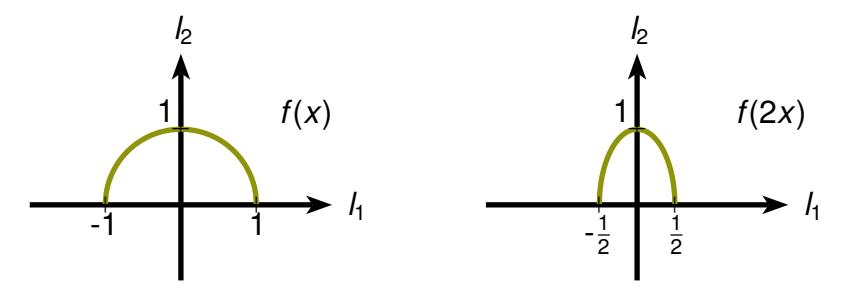
\includegraphics[width=0.55\textwidth]{img/_page_142_Figure_6.jpeg}
\end{center}
\end{ejemplo}

\subsection{Reflexión respecto al eje $Y$: $f(-x)$}

Si $g(x) = f(-x)$, el gráfico de $g$ es el reflejo del gráfico de $f$ respecto
al eje $Y$: si $(-x,y) \in f$ entonces $(x,y) \in g$.

\begin{ejemplo}
Sean $f(x) = 2x+5$ y $g(x) = f(-x) = -2x+5$. El gráfico de $g$ es el reflejo
del de $f$ respecto al eje $Y$.

\begin{center}
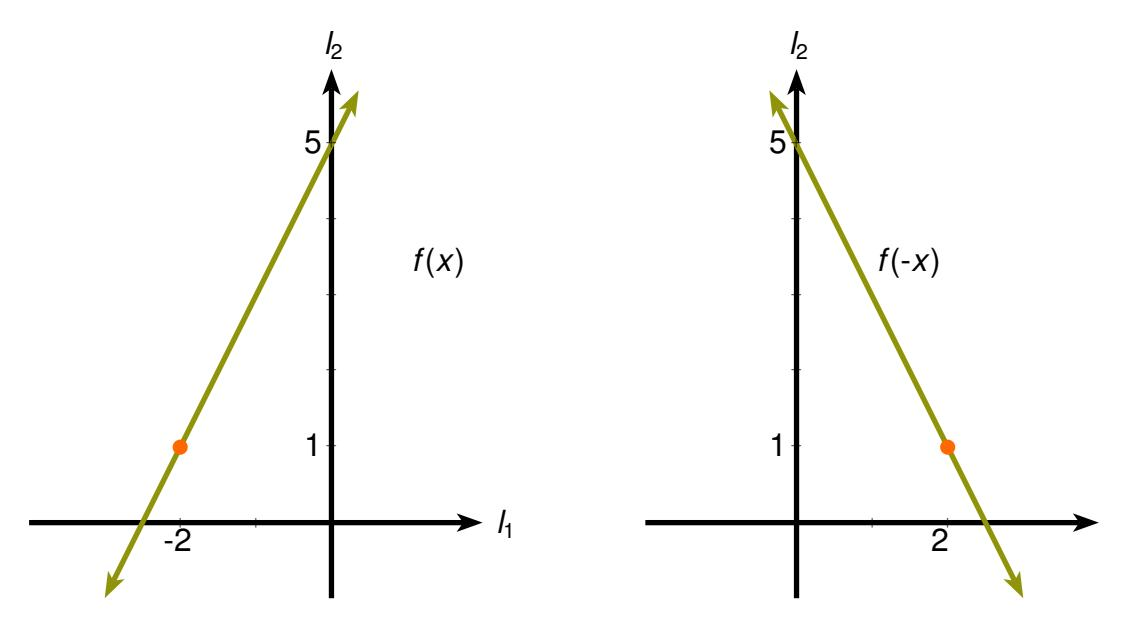
\includegraphics[width=0.55\textwidth]{img/_page_142_Figure_12.jpeg}
\end{center}
\end{ejemplo}

\begin{observacion}
Estas transformaciones se pueden combinar. Por ejemplo, para graficar
$h(x) = c\,f(x-a)+b$ conviene partir del gráfico de $f$, trasladarlo $a$
unidades horizontalmente, escalarlo verticalmente en un factor $c$ y finalmente
trasladarlo $b$ unidades verticalmente, en ese orden.
\end{observacion}

\section{Gráfica de funciones racionales}

Estudiamos ahora el gráfico de dos funciones racionales sencillas, que servirán
de modelo para otras funciones de la forma $\frac{1}{x^n}$.

\subsection{La función $f(x) = \dfrac{1}{x}$}

Sea $f(x) = \dfrac{1}{x}$. Tenemos $\mathsf{Dom}\,f = \mathbb{R}-\{0\}$ y
$\mathsf{Rec}\,f = \mathbb{R}-\{0\}$. Como $0 \notin \mathsf{Dom}\,f$ y
$f(x)\neq 0$ para todo $x$, el gráfico de $f$ no intersecta a los ejes $X$ ni
$Y$.

Además, $f(x) > 0 \leftrightarrow x>0$ y $f(x)<0 \leftrightarrow x<0$: $f$ es
positiva en $]0,\infty[$ y negativa en $]-\infty,0[$.

Como $f(-x) = \dfrac{1}{-x} = -\dfrac{1}{x} = -f(x)$, la función es impar, así
que basta estudiarla en $]0,\infty[$ y luego extender por simetría respecto al
origen.

Si $x,y \in [0,\infty[$ y $x<y$ entonces $\dfrac{1}{x} > \dfrac{1}{y}$, de donde
$f$ es estrictamente decreciente en $[0,\infty[$. Tampoco está acotada
superiormente en ese intervalo: si $x>0$ y $\varepsilon$ es tal que
$x-\varepsilon>0$, entonces $\dfrac{1}{x-\varepsilon} > \dfrac{1}{x}$.

\begin{center}
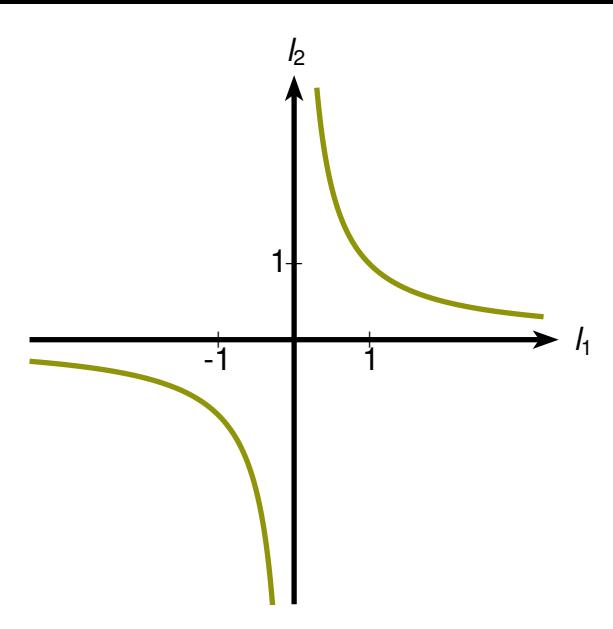
\includegraphics[width=0.5\textwidth]{img/_page_136_Figure_3.jpeg}
\end{center}

La función es uno a uno y su inversa es $f^{-1}(x) = \dfrac{1}{x}$, es decir,
$f$ coincide con su propia inversa.

\subsection{La función $f(x) = \dfrac{1}{x^2}$}

Sea $f(x) = \dfrac{1}{x^2}$. Tenemos $\mathsf{Dom}\,f = \mathbb{R}-\{0\}$ y
$\mathsf{Rec}\,f = \mathbb{R}^+$.

Como $f(-x) = \dfrac{1}{(-x)^2} = \dfrac{1}{x^2} = f(x)$, la función es par, así
que basta estudiarla en $[0,\infty[$.

En $[0,\infty[$, $f(x) = \dfrac{1}{x^2} > 0$, así que $f$ es positiva ahí. Si
$x<y$ (ambos en $[0,\infty[$) entonces $\dfrac{1}{x^2} > \dfrac{1}{y^2}$, luego
$f$ es estrictamente decreciente en $[0,\infty[$. Tampoco está acotada
superiormente: si $x>0$ y $x-\varepsilon>0$, entonces
$\dfrac{1}{(x-\varepsilon)^2} > \dfrac{1}{x^2}$.

\begin{center}
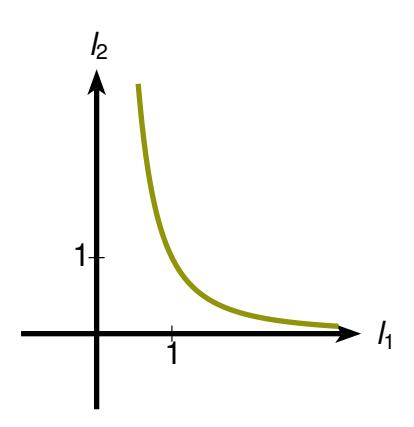
\includegraphics[width=0.48\textwidth]{img/_page_137_Figure_2.jpeg}
\end{center}

Extendiendo por paridad a todo $\mathbb{R}$:

\begin{center}
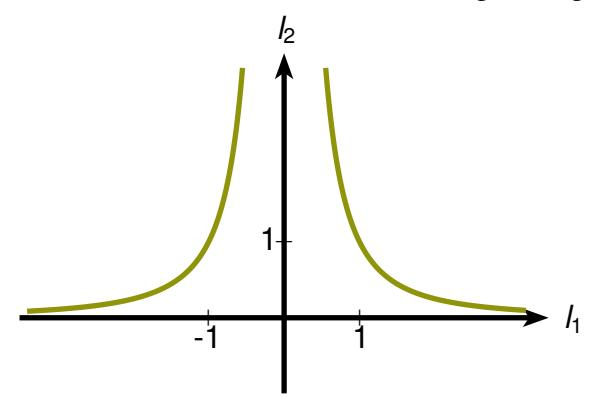
\includegraphics[width=0.5\textwidth]{img/_page_137_Figure_5.jpeg}
\end{center}

A diferencia de $\dfrac{1}{x}$, esta función no es uno a uno (por ejemplo,
$f(1)=f(-1)=1$).

\begin{observacion}
En ambos casos, el eje $Y$ (la recta $x=0$) y el eje $X$ (la recta $y=0$, solo
para $\dfrac{1}{x^2}$) actúan como ``barreras'' que el gráfico se acerca sin
tocar: esto es lo que más adelante se estudiará formalmente como asíntotas.
Por ahora basta con reconocer este comportamiento a partir del análisis de
signo, paridad y monotonía, como en los ejemplos anteriores.
\end{observacion}

\end{document}
